% BLG483E - HW3 Technical Report (English)
% Local Wikipedia RAG Assistant
%
% Build (run twice for stable TOC):
%   pdflatex BLG483E_HW3_rapor.tex
%   pdflatex BLG483E_HW3_rapor.tex

\documentclass[11pt,a4paper]{article}

\usepackage[utf8]{inputenc}
\usepackage[T1]{fontenc}
\usepackage[english]{babel}

\usepackage{geometry}
\usepackage{hyperref}
\usepackage{enumitem}
\usepackage{booktabs}
\usepackage{graphicx}
\usepackage{xcolor}
\usepackage{listings}
\usepackage{tikz}
\usetikzlibrary{arrows.meta,positioning}

\geometry{margin=2.5cm}
\hypersetup{colorlinks=true, linkcolor=blue, urlcolor=blue}

\definecolor{codegreen}{rgb}{0,0.5,0}
\lstdefinestyle{pythonstyle}{
  language=Python,
  basicstyle=\ttfamily\footnotesize,
  keywordstyle=\color{blue}\bfseries,
  commentstyle=\color{codegreen},
  stringstyle=\color{orange!80!black},
  breaklines=true,
  frame=single,
  columns=fullflexible,
  showstringspaces=false,
  tabsize=4,
  numbers=left,
  numberstyle=\tiny\color{gray},
  xleftmargin=1.5em,
}
\lstset{style=pythonstyle}

\title{\textbf{BLG483E -- Homework 3}\\[0.5em]
\Large Local Wikipedia RAG Assistant:\\
Technical Report and Code Walkthrough}
\author{Name / Student ID: \texttt{[FILL IN]}}
\date{\today}

\begin{document}
\maketitle

\begin{abstract}
This report documents a fully \emph{local} Retrieval-Augmented Generation (RAG) assistant
that answers questions about famous people and places using Wikipedia-derived text.
The system ingests English Wikipedia extracts, splits them into overlapping chunks,
embeds them with a local \texttt{sentence-transformers} model, stores vectors in a
persistent Chroma database with metadata, routes queries to \texttt{person} and/or
\texttt{place} scopes, and generates answers with a local Ollama LLM without any
external LLM API. The report explains each source file, the end-to-end execution path,
and representative code fragments that illustrate how the implementation works.
\end{abstract}

\tableofcontents
\newpage

%==============================================================================
\section{Introduction and assignment goals}
%==============================================================================

The course homework (BLG483E HW3) requires building a simplified ChatGPT-like system that:
\begin{itemize}[leftmargin=*]
  \item runs entirely on the student's machine (localhost);
  \item ingests Wikipedia pages for at least 20 people and 20 places, including a mandatory minimum set;
  \item defines a chunking strategy for large documents;
  \item uses \emph{local} embeddings and a vector database;
  \item classifies whether a question targets a person, a place, or both, and retrieves accordingly;
  \item uses a \emph{local} language model to answer from retrieved context and to say
        \texttt{I don't know} when the context is insufficient;
  \item provides a simple chat UI or CLI.
\end{itemize}

This implementation satisfies these requirements using Python, SQLite for structured
ingestion records, Chroma for vector search, SentenceTransformers for embeddings, and
Ollama for local generation.

%==============================================================================
\section{Repository layout and module responsibilities}
%==============================================================================

Table~\ref{tab:modules} summarizes the main Python modules and their roles.

\begin{table}[h]
\centering
\begin{tabular}{@{}p{3.2cm}p{10.8cm}@{}}
\toprule
\textbf{File} & \textbf{Responsibility} \\
\midrule
\texttt{config.py} &
Central configuration: filesystem paths, Wikipedia API URL and headers, embedding model id,
Ollama model id, chunk size/overlap, and retrieval \texttt{TOP\_K}. \\
\texttt{entities.py} &
Curated lists \texttt{PEOPLE} and \texttt{PLACES} (each at least 20 entries), including the
homework-required minimum entities. \\
\texttt{chunk\_row.py} &
\texttt{TypedDict} describing one chunk row passed from ingestion to the vector store. \\
\texttt{chunking.py} &
Deterministic sliding-window chunking with overlap on normalized plaintext. \\
\texttt{wikipedia\_ingest.py} &
Fetches Wikipedia extracts, persists \texttt{docs}/\texttt{chunks} in SQLite, returns a list of
\texttt{ChunkRow} objects for embedding. \\
\texttt{vector\_store.py} &
Chroma persistent client, embedding, upsert, metadata-filtered query, and resilient reset. \\
\texttt{retrieval.py} &
Rule-based query classification, Chroma retrieval, and SQLite keyword fallback if Chroma fails. \\
\texttt{generation.py} &
Ollama chat completion with a strict system prompt for grounded answers. \\
\texttt{main.py} &
Interactive CLI loop: commands and question answering with optional source printing. \\
\texttt{ingest.py} &
One-shot pipeline for demo/reset: reset store, verbose ingest, upsert to Chroma. \\
\bottomrule
\end{tabular}
\caption{Main Python modules and responsibilities.}
\label{tab:modules}
\end{table}

\noindent
Additional deliverable documents (not Python) include \texttt{README.md},
\texttt{Product\_prd.md}, and \texttt{recommendation.md}.

%==============================================================================
\section{End-to-end system architecture}
%==============================================================================

Figure~\ref{fig:flow} shows the logical pipeline from ingestion to answer generation.

\begin{figure}[h]
\centering
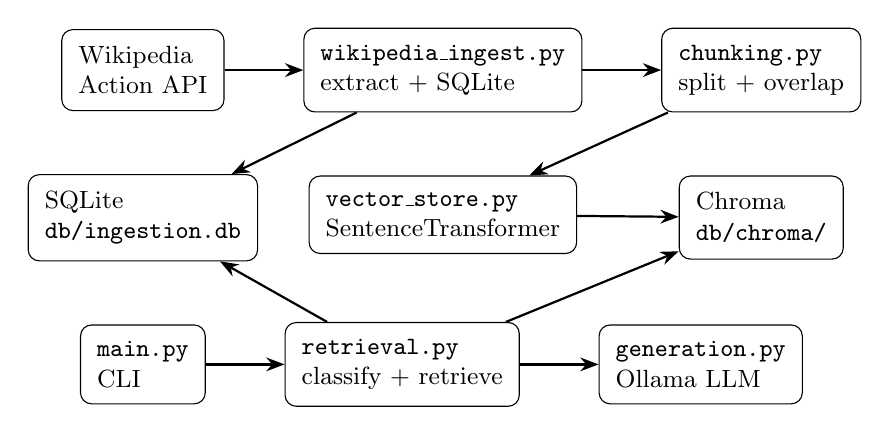
\begin{tikzpicture}[
  node distance=8mm and 10mm,
  box/.style={draw, rounded corners, align=left, inner sep=6pt, font=\small},
  arr/.style={-{Stealth}, thick},
]
\node[box] (wiki) {Wikipedia\\Action API};
\node[box, right=of wiki] (ingest) {\texttt{wikipedia\_ingest.py}\\extract + SQLite};
\node[box, right=of ingest] (chunk) {\texttt{chunking.py}\\split + overlap};
\node[box, below=of wiki] (sqlite) {SQLite\\\texttt{db/ingestion.db}};
\node[box, below=of ingest] (emb) {\texttt{vector\_store.py}\\SentenceTransformer};
\node[box, below=of chunk] (chroma) {Chroma\\\texttt{db/chroma/}};
\node[box, below=of sqlite] (cli) {\texttt{main.py}\\CLI};
\node[box, right=of cli] (retr) {\texttt{retrieval.py}\\classify + retrieve};
\node[box, right=of retr] (llm) {\texttt{generation.py}\\Ollama LLM};

\draw[arr] (wiki) -- (ingest);
\draw[arr] (ingest) -- (chunk);
\draw[arr] (ingest) -- (sqlite);
\draw[arr] (chunk) -- (emb);
\draw[arr] (emb) -- (chroma);
\draw[arr] (cli) -- (retr);
\draw[arr] (retr) -- (chroma);
\draw[arr] (retr) -- (sqlite);
\draw[arr] (retr) -- (llm);
\end{tikzpicture}
\caption{High-level data flow: Wikipedia $\rightarrow$ SQLite chunks $\rightarrow$ embeddings $\rightarrow$
Chroma; user query $\rightarrow$ retrieval (Chroma with optional SQLite fallback) $\rightarrow$ Ollama.}
\label{fig:flow}
\end{figure}

\subsection{Runtime artifacts on disk}
\begin{itemize}[leftmargin=*]
  \item \texttt{db/ingestion.db}: SQLite tables \texttt{docs} (one row per Wikipedia page) and
        \texttt{chunks} (one row per chunk), enabling provenance and fallback retrieval.
  \item \texttt{db/chroma/}: Chroma persistent vector index and metadata for approximate
        nearest-neighbor search.
  \item \texttt{data/}: reserved directory for auxiliary local files (if needed).
\end{itemize}

%==============================================================================
\section{Configuration layer (\texttt{config.py})}
%==============================================================================

All ``magic constants'' live in \texttt{config.py} so the rest of the codebase stays readable
and reproducible. Listing~\ref{lst:config} shows the essential settings.

\begin{lstlisting}[caption={Central paths and model identifiers (\texttt{config.py}).},label={lst:config}]
from pathlib import Path

BASE_DIR = Path(__file__).resolve().parent
DATA_DIR = BASE_DIR / "data"
DB_DIR = BASE_DIR / "db"
CHROMA_DIR = DB_DIR / "chroma"
SQLITE_PATH = DB_DIR / "ingestion.db"

EMBEDDING_MODEL = "sentence-transformers/all-MiniLM-L6-v2"
OLLAMA_MODEL = "llama3.2:3b"

CHUNK_SIZE = 750
CHUNK_OVERLAP = 120
TOP_K = 5

WIKIPEDIA_API = "https://en.wikipedia.org/w/api.php"
WIKIPEDIA_HEADERS = {
    "User-Agent": "BLG483E-LocalWikipediaRAG/1.0 (course homework; Python requests)",
    "Accept": "application/json",
}
\end{lstlisting}

\paragraph{Why \texttt{WIKIPEDIA\_HEADERS}?}
Wikimedia commonly rejects anonymous \texttt{requests} calls without a descriptive
\texttt{User-Agent}. Without it, ingestion may fail with HTTP 403, producing empty chunks.

%==============================================================================
\section{Entity inventory (\texttt{entities.py})}
%==============================================================================

The homework requires at least 20 people and 20 places, including a fixed minimum subset.
The project encodes these as two Python lists, \texttt{PEOPLE} and \texttt{PLACES}.
During ingestion, each title is paired with a label \texttt{entity\_type} $\in$
\{\texttt{person}, \texttt{place}\}, which later drives metadata filtering during retrieval.

%==============================================================================
\section{Chunk schema (\texttt{chunk\_row.py})}
%==============================================================================

Chunks are the atomic units stored in Chroma. A \texttt{ChunkRow} is a \texttt{TypedDict}
ensuring consistent keys and value types between ingestion and \texttt{vector\_store.py}:

\begin{lstlisting}[caption={Chunk record schema (\texttt{chunk\_row.py}).},label={lst:chunkrow}]
from typing import TypedDict

class ChunkRow(TypedDict):
    id: str
    title: str
    entity_type: str
    source_url: str
    chunk_index: int
    text: str
\end{lstlisting}

\noindent
The \texttt{id} is a deterministic string key such as \texttt{person:Albert Einstein:0},
which makes upserts idempotent and debuggable.

%==============================================================================
\section{Chunking strategy (\texttt{chunking.py})}
%==============================================================================

Wikipedia extracts can be very long. The chunker:
\begin{enumerate}[leftmargin=*]
  \item collapses whitespace to single spaces (normalization);
  \item slides a window of length \texttt{CHUNK\_SIZE} characters;
  \item advances the window by \texttt{step = max(1, CHUNK\_SIZE - CHUNK\_OVERLAP)} so consecutive
        chunks overlap by \texttt{CHUNK\_OVERLAP} characters.
\end{enumerate}

\begin{lstlisting}[caption={Sliding-window chunking with overlap (\texttt{chunking.py}).},label={lst:chunking}]
def chunk_text(text: str, chunk_size: int, overlap: int) -> List[str]:
    cleaned = " ".join(text.split())
    if not cleaned:
        return []

    chunks: List[str] = []
    start = 0
    step = max(1, chunk_size - overlap)
    while start < len(cleaned):
        end = start + chunk_size
        chunk = cleaned[start:end].strip()
        if chunk:
            chunks.append(chunk)
        start += step
    return chunks
\end{lstlisting}

\paragraph{Design rationale.}
Overlap reduces the chance that an important sentence sits on a chunk boundary and becomes
weakly represented in both neighboring chunks for embedding and retrieval.

%==============================================================================
\section{Wikipedia ingestion and SQLite persistence (\texttt{wikipedia\_ingest.py})}
%==============================================================================

\subsection{API call and robustness}
The module calls the Wikipedia \texttt{query} API with \texttt{prop=extracts} and
\texttt{explaintext=1} to retrieve plain-text extracts (not HTML). Network failures and
transient HTTP errors are handled with retries and exponential backoff-style sleep for
status codes like 429 and certain 5xx responses.

\begin{lstlisting}[caption={Wikipedia fetch with retries (\texttt{wikipedia\_ingest.py}, excerpt).},label={lst:wiki}]
def fetch_wikipedia_extract(title: str) -> Tuple[str, str]:
    params = {
        "action": "query",
        "format": "json",
        "prop": "extracts",
        "explaintext": 1,
        "redirects": 1,
        "titles": title,
    }
    for attempt in range(6):
        try:
            response = requests.get(
                WIKIPEDIA_API, params=params, headers=WIKIPEDIA_HEADERS, timeout=30
            )
            response.raise_for_status()
            data = response.json()
            pages = data["query"]["pages"]
            page = next(iter(pages.values()))
            extract = page.get("extract", "")
            page_title = page.get("title", title)
            source_url = f"https://en.wikipedia.org/wiki/{page_title.replace(' ', '_')}"
            return extract, source_url
        except requests.HTTPError as exc:
            status = exc.response.status_code if exc.response is not None else None
            if status not in (429, 500, 502, 503, 504) or attempt == 5:
                raise
            time.sleep(1.0 * (attempt + 1))
        except requests.RequestException as exc:
            if attempt == 5:
                raise
            time.sleep(1.0 * (attempt + 1))
\end{lstlisting}

\subsection{SQLite schema}
Two tables are maintained:
\begin{itemize}[leftmargin=*]
  \item \texttt{docs}: one row per ingested page with \texttt{title} (primary key),
        \texttt{entity\_type}, canonical \texttt{source\_url}, and \texttt{text\_length}.
  \item \texttt{chunks}: one row per chunk with stable \texttt{id}, foreign linkage via
        \texttt{title} + \texttt{entity\_type}, \texttt{chunk\_index}, and \texttt{text}.
\end{itemize}

\noindent
At the start of each full ingest, the implementation clears prior SQLite rows so a failed
partial ingest cannot leave misleading ``person-only'' residue when places were skipped.

\subsection{Corpus builder output}
\texttt{build\_local\_corpus} returns a flat list of \texttt{ChunkRow} dictionaries suitable
for immediate embedding and upsert. Optional \texttt{verbose=True} prints per-entity progress
and a final success/failure summary for demos and debugging.

%==============================================================================
\section{Vector store: embeddings and Chroma (\texttt{vector\_store.py})}
%==============================================================================

\subsection{Class \texttt{LocalVectorStore}}
On construction, the class:
\begin{itemize}[leftmargin=*]
  \item ensures \texttt{CHROMA\_DIR} exists;
  \item creates a \texttt{chromadb.PersistentClient} pointing at that directory;
  \item opens (or creates) a single collection named \texttt{wiki\_chunks};
  \item loads \texttt{SentenceTransformer(EMBEDDING\_MODEL)} once (this can dominate startup time).
\end{itemize}

\subsection{Upsert pipeline}
\texttt{upsert\_rows} embeds all chunk texts in batch, builds parallel lists of \texttt{ids},
\texttt{embeddings}, \texttt{documents}, and \texttt{metadatas}, then calls Chroma
\texttt{collection.upsert}. Metadata includes \texttt{entity\_type} for homework-compliant filtering.

\begin{lstlisting}[caption={Embedding batch and upsert (\texttt{vector\_store.py}, excerpt).},label={lst:upsert}]
def upsert_rows(self, rows: List[ChunkRow]) -> None:
    if not rows:
        return
    texts = [r["text"] for r in rows]
    embeddings = self.embedder.encode(texts, show_progress_bar=True).tolist()
    ids = [r["id"] for r in rows]
    metadatas: List[Metadata] = [
        cast(Metadata, {
            "title": r["title"],
            "entity_type": r["entity_type"],
            "source_url": r["source_url"],
            "chunk_index": r["chunk_index"],
        })
        for r in rows
    ]
    try:
        self.collection.upsert(
            ids=ids, embeddings=embeddings, documents=texts, metadatas=metadatas,
        )
    except Exception:
        self.reset()
        self.collection.upsert(
            ids=ids, embeddings=embeddings, documents=texts, metadatas=metadatas,
        )
\end{lstlisting}

\subsection{Metadata-filtered vector query}
The homework requires retrieving from the correct ``store'' or applying filtering.
This project uses \textbf{Option B}: one collection with \texttt{entity\_type} metadata.
The query builds a Chroma \texttt{where} clause:
\begin{itemize}[leftmargin=*]
  \item single filter: \texttt{\{"entity\_type": "person"\}} or \texttt{"place"};
  \item combined filter: \texttt{\{"\$or": [\{"entity\_type": "person"\}, \{"entity\_type": "place"\}]\}}.
\end{itemize}

\subsection{Resilience: reset and index corruption}
Some environments can corrupt on-disk HNSW segments. \texttt{reset()} attempts a normal
collection delete/recreate, and if the collection is still unreadable it deletes the
entire \texttt{CHROMA\_DIR} and reinitializes the client. \texttt{upsert\_rows} retries once
after \texttt{reset()} on upsert failure.

%==============================================================================
\section{Retrieval and query routing (\texttt{retrieval.py})}
%==============================================================================

\subsection{Rule-based classification (\texttt{classify\_query})}
The classifier is intentionally simple (homework-allowed): it checks whether the query
contains known entity titles from \texttt{PEOPLE}/\texttt{PLACES}, and also checks small
keyword hint sets (e.g., ``where'' suggests a place, ``who'' suggests a person). If both
signals appear, retrieval widens to both entity types.

\begin{lstlisting}[caption={Query routing logic (\texttt{retrieval.py}, excerpt).},label={lst:classify}]
def classify_query(query: str) -> List[str]:
    q = query.lower()
    has_person_name = any(name.lower() in q for name in PEOPLE)
    has_place_name = any(name.lower() in q for name in PLACES)
    has_person_hint = any(word in q for word in PERSON_HINTS)
    has_place_hint = any(word in q for word in PLACE_HINTS)

    if (has_person_name and has_place_name) or (has_person_hint and has_place_hint):
        return ["person", "place"]
    if has_person_name or has_person_hint:
        return ["person"]
    if has_place_name or has_place_hint:
        return ["place"]
    return ["person", "place"]
\end{lstlisting}

\subsection{Primary retrieval (\texttt{retrieve\_context})}
\texttt{retrieve\_context} calls \texttt{store.query} with the user question as the query
text, embedding it with the same model used at ingest time (required for meaningful ANN
search). Returned documents are concatenated into a numbered context string for the LLM.

\subsection{SQLite fallback retrieval}
If Chroma raises \texttt{RuntimeError} (unreadable index), the module falls back to SQLite:
it loads candidate chunks filtered by \texttt{entity\_type}, scores them with a lightweight
token overlap heuristic between query and chunk text (plus a title match boost), and
returns the top-\texttt{TOP\_K} chunks. This preserves demo functionality even when the
vector index is unstable.

%==============================================================================
\section{Local answer generation (\texttt{generation.py})}
%==============================================================================

The generator uses the Ollama Python client with a low temperature. The system prompt
forces grounding: answers must come only from the provided context; if insufficient, the
model should output \texttt{I don't know}. The code also short-circuits empty context and
handles Ollama failures safely.

\begin{lstlisting}[caption={Grounded generation with Ollama (\texttt{generation.py}).},label={lst:gen}]
def generate_answer(query: str, context: str) -> str:
    if not context.strip():
        return "I don't know"

    prompt = (
        f"Context:\n{context}\n\n"
        f"Question: {query}\n"
        "Answer using only context."
    )
    try:
        response = ollama.chat(
            model=OLLAMA_MODEL,
            messages=[
                {"role": "system", "content": SYSTEM_PROMPT},
                {"role": "user", "content": prompt},
            ],
            options={"temperature": 0.1},
        )
    except Exception:
        return "I don't know"

    answer = response["message"]["content"].strip()
    return answer or "I don't know"
\end{lstlisting}

%==============================================================================
\section{Command-line interface (\texttt{main.py})}
%==============================================================================

\texttt{main.py} implements the interactive loop shown in Listing~\ref{lst:main}.
Commands are explicit slash-commands; any other input is treated as a question.

\begin{lstlisting}[caption={CLI control flow (\texttt{main.py}, excerpt).},label={lst:main}]
store = LocalVectorStore()
show_sources = False

while True:
    user_input = input("\nYou> ").strip()
    if user_input == "/quit":
        break
    if user_input == "/sources":
        show_sources = not show_sources
        continue
    if user_input == "/reset":
        store.reset()
        continue
    if user_input == "/ingest":
        rows = build_local_corpus()
        if not rows:
            print("Ingestion produced 0 chunks. Likely Wikipedia rate-limit (HTTP 429).")
            continue
        store.upsert_rows(rows)
        continue

    context, sources = retrieve_context(store, user_input)
    answer = generate_answer(user_input, context)
    print(f"Assistant> {answer}")
    if show_sources and sources:
        ...
\end{lstlisting}

%==============================================================================
\section{One-shot ingestion script (\texttt{ingest.py})}
%==============================================================================

For reproducible demos, \texttt{ingest.py} performs a clean sequence: reset the vector store,
run verbose ingestion, then upsert all rows. This avoids partially stale Chroma state when
re-recording a video.

\begin{lstlisting}[caption={Batch ingest entrypoint (\texttt{ingest.py}).},label={lst:ingest}]
def main() -> None:
    store = LocalVectorStore()
    print("Resetting vector store before fresh ingest...")
    store.reset()
    rows = build_local_corpus(verbose=True)
    if not rows:
        print("No chunks were prepared. Retry ingest after a short wait.")
        return
    print("\nEmbedding + upsert to Chroma...")
    store.upsert_rows(rows)
    print(f"Done. Stored {len(rows)} chunks in vector store.")
\end{lstlisting}

%==============================================================================
\section{How to run (reproducible checklist)}
%==============================================================================

\begin{enumerate}[leftmargin=*]
  \item Create and activate a virtual environment.
  \item \texttt{pip install -r requirements.txt}
  \item Install Ollama and pull the configured chat model, e.g.\ \texttt{ollama pull llama3.2:3b}.
  \item Run \texttt{python ingest.py} (recommended for a clean ingest + upsert), or start
        \texttt{python main.py} and use \texttt{/ingest}.
  \item Start \texttt{python main.py}, optionally enable \texttt{/sources}, and ask questions.
\end{enumerate}

%==============================================================================
\section{Design decisions and trade-offs}
%==============================================================================

\paragraph{Option B: single vector store with metadata.}
Using one Chroma collection with \texttt{entity\_type} simplifies maintenance and naturally
supports mixed queries with a single query path, while still allowing metadata filtering.

\paragraph{Local embeddings vs.\ Ollama embeddings.}
The project uses SentenceTransformers for embeddings (homework-allowed) for stable offline
behavior and reproducible vector geometry independent of Ollama embedding endpoints.

\paragraph{Rule-based routing vs.\ learned routing.}
The classifier is explainable and fast, but can mis-route ambiguous queries; widening filters
to both types reduces false negatives at the cost of extra retrieved noise.

\paragraph{LLM grounding vs.\ comparison questions.}
Comparison answers depend on whether retrieved chunks jointly contain comparable facts; the
system prompt encourages abstaining (\texttt{I don't know}) when the context does not support
a direct comparison.

%==============================================================================
\section{Limitations and known failure modes}
%==============================================================================

\begin{itemize}[leftmargin=*]
  \item \textbf{Wikipedia rate limits:} aggressive repeated ingestion can yield HTTP 429;
        the code retries, but the user may still need to wait and re-run.
  \item \textbf{Incomplete ingestion:} if many pages fail, downstream answers may be wrong
        or empty for missing entities.
  \item \textbf{Chroma disk corruption:} rare but possible; reset/rebuild mitigates it, and
        SQLite fallback improves availability for Q\&A demos.
  \item \textbf{Retrieval quality:} small \texttt{TOP\_K}, chunk boundaries, and embedding model
        capacity limit recall and precision.
\end{itemize}

%==============================================================================
\section{Conclusion}
%==============================================================================

This project combines retrieval and generation into a single local-first assistant aligned
with the homework constraints: Wikipedia ingestion, chunking, local embeddings, metadata-aware
vector search, simple query routing, and Ollama-based grounded answers with an explicit
unknown response policy. The modular layout maps cleanly to the RAG lifecycle and is
documented here with representative code excerpts illustrating the runtime behavior.

\vfill
\noindent\textit{This report describes the repository at the time of writing; behavior should
always be verified against the latest source code.}

\end{document}
